\chapter{Sources et Évolution de la mécanique quantique}
\section{Loi de Planck}
\begin{de}
Une onde de fréquence $\upsilon$ peut être représenter comme une paquet de photons. Chaque photons possède une énergie E définie par :
$$E = h\upsilon$$
Avec h, la constante de Planck :
$$h=6,62.10^{-34} J.s$$
On introduit aussi $\hbar$, défini par : 
$$\hbar = \dfrac{h}{2\pi}$$
Or comme : $\lambda = CT$, on obtient : 
$$E = \dfrac{hC}{\lambda}$$
Cette énergie est exprimé en Joules
\end{de}
\section{Formule de Ritz}
Soit $\sigma=\dfrac{1}{\lambda}$ le nombre d'onde. La formule de Ritz est : 
$$\sigma = R_H(\dfrac{1}{n^2}-\dfrac{1}{m^2})$$
Avec :
\[\left\{\begin{array}{l}
  R_H = 10979708~ m^{-1}\\
  n : \mbox{ Le nombre principale de la série (ex : 2 pour l'hydrogène)}\\
  m : \mbox{ Entier superieur à n, que l'on fait varier pour trouver la série : m=n+1,m=n+2 .... }
  \end{array}\right.
\]
\section{Énergie de l'atome d'hydrogène}
\begin{de}
 En utilisant comme unité l'électron volt défini par : 1eV = 1,6.$10^{-19}$ J, on obtient l'énergie de l'atome dans un niveau n :
$$E_n = -\dfrac{13.6}{n^2}$$
n est appelé nombre quantique principal.
\end{de}
\section{Énergie d'un ion hydrogénoïde}
\begin{de}
 Un ion hydrogénoïde est un édifice monoatomique monoélectrique, donc qui ne comporte plus qu'un seul électron.
\end{de}
On défini les relations suivants pour ce type d'ion :
\[\left\{\begin{array}{c}
  E_n = -13.6\left(\dfrac{Z}{n}\right)^2 \\
  r_n = n^2\left(\dfrac{a_0}{Z}\right) 
  \end{array}\right.
\]
Avec :
\[\left\{\begin{array}{l}
   \mbox{ Z = Nombre de charge du noyau} \\
   a_0 = \mbox{ Rayon de Bohr }
  \end{array}\right.
\]
\section{Longueur d'onde de Broglie}
\begin{de}
 On défini la longueur d'onde de Broglie pour tous corpuscules en mouvement par :
$$\lambda_{dB} = \dfrac{h}{p}$$
Avec p la quantité de mouvement du corpuscule.
\end{de}
\chapter{Fonctions d'onde, nombres quantiques}
\section{Fonction d'onde}
\begin{de}
 Une fonction d'onde est défini comme une solution de l'équation de Schrodinger. Cette variable est une variable d'espace, elle oblige donc l'existence de trois paramètres, appelé nombres quantiques
\end{de}
Pour une valeur donnée de n, il existe $n^2$ fonctions d'ondes. On dit que le niveau d'énergie est dégénéré de degrès $n^2$
\section{Nombres quantiques}
\subsection{Nombre quantique principal}
Ce nombre quantique quantifie l'énergie, il est noté n. Il est utilisé dans la quantification de l'énergie d'un ion hydrogénoïde.
\subsection{Nombre quantique orbital}
Ce nombre quantique quantifie le moment cinétique, il est noté l. En mécanique quantique, le module du moment cinétique est : 
$$L^2=l(l+1)\hbar^2$$
Il ne peut prendre que certaines valeurs :
$$0 \leq l \leq n-1$$
\subsection{Nombre quantique magnétique}
Ce nombre quantique, noté ml, quantifie la projection d'un moment cinétique sur un champ magnétique $\vec B$ extérieur. Soit $L_z$ la projection du moment cinétique sur l'axe z'z : 
$$L_z = ml\hbar$$
Les valeurs que peu prendre ml sont : 
$$-l \leq ml \leq l$$
\subsection{Spin}
Ce nombre quantique, noté ms, quantifie le moment cinétique intrinsèque de l'électron. Il ne peut prendre comme valeur que $\pm \dfrac{1}{2}$\\
La quadriplet suivant (n,l,ml,ms) défini un état quantique. À une valeur de n correspond $2n^2$ états quantitique
\section{Orbitale atomique}
On associe aux différentes valeurs du nombre quantique l une lettre :
\begin{center}
% use packages: array
\begin{tabular}{|l|l|l|l|l|l|}
\hline
l & 0 & 1 & 2 & 3 & 4 \\ \hline
Lettre & s & p & d & f & g \\ \hline
\end{tabular}
\end{center}
On obtient l'écriture suivante :
$$\psi_{(n,l,ml)}=n.Lettre_{ml}$$
Ex :
$$\psi_{(3,1,-1)}=3p_{-1}$$
\chapter{Atomes polyélectroniques}
Un système peut être caractérisé dans la mécanique quantique par le quadruplet (n,l,ml,ms)
\section{Règle de Klechkowski}
Ce règle défini la façon de rempli les orbitales orbitale atomique. 
%\begin{figure}[ht]
%  \centering
%  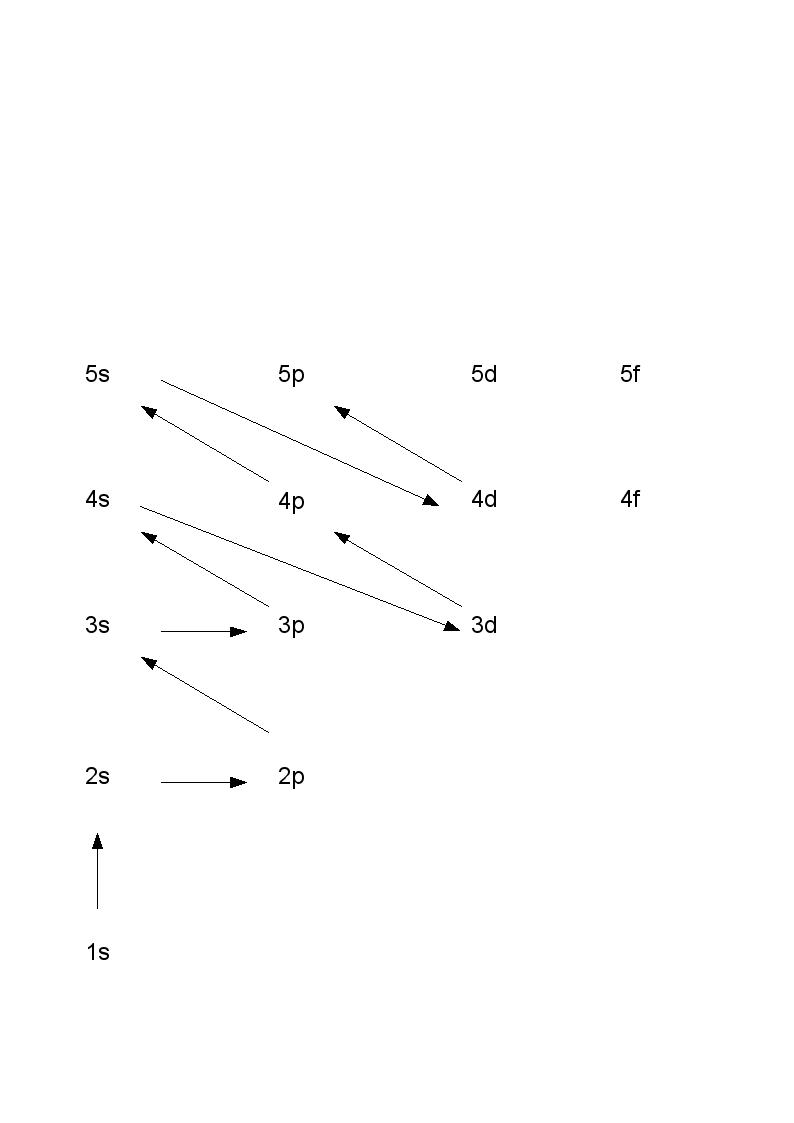
\includegraphics[width=6cm]{Klech.jpg}
%  \caption{Illustration de la règle de Klechkowski}
%\end{figure}
\section{Configuration électronique d'un atome}
\subsection{Principe de stabilité}
\begin{enon}
 Connaissant l'évolution des niveaux énergétiques des différentes O.A. d'un atome à N électrons, le remplissage des O.A. se fait dans le sens des énergies croissantes.
\end{enon}
\subsection{Principe d'exclusion de Pauli}
\begin{enon}
 Dans un atome polyélectronique, deux électrons ne peuvent être dans le même état quantique
\end{enon}
Ceci implique que sur chaque O.A, on peut mettre au maximum deux électrons antiparallèle
\subsection{Principe de Hund}
\begin{enon}
 Quand on place des électrons dans des O.A. dégénérées, les électrons occupent un  maximum d'O.A. avec des spins parallèles. C'est seulement quand tout les O.A. sont occupé par des spins parallèle que l'on rajoute des électrons en spin antiparallèle.
\end{enon}
\subsection{Configuration électronique}
Considerons l'atome d'oxygène (Z = 8) dans son êtat fondamental, on peut établir le diagramme énergétique suivant :
%\begin{figure}[!h]
%  \centering
%  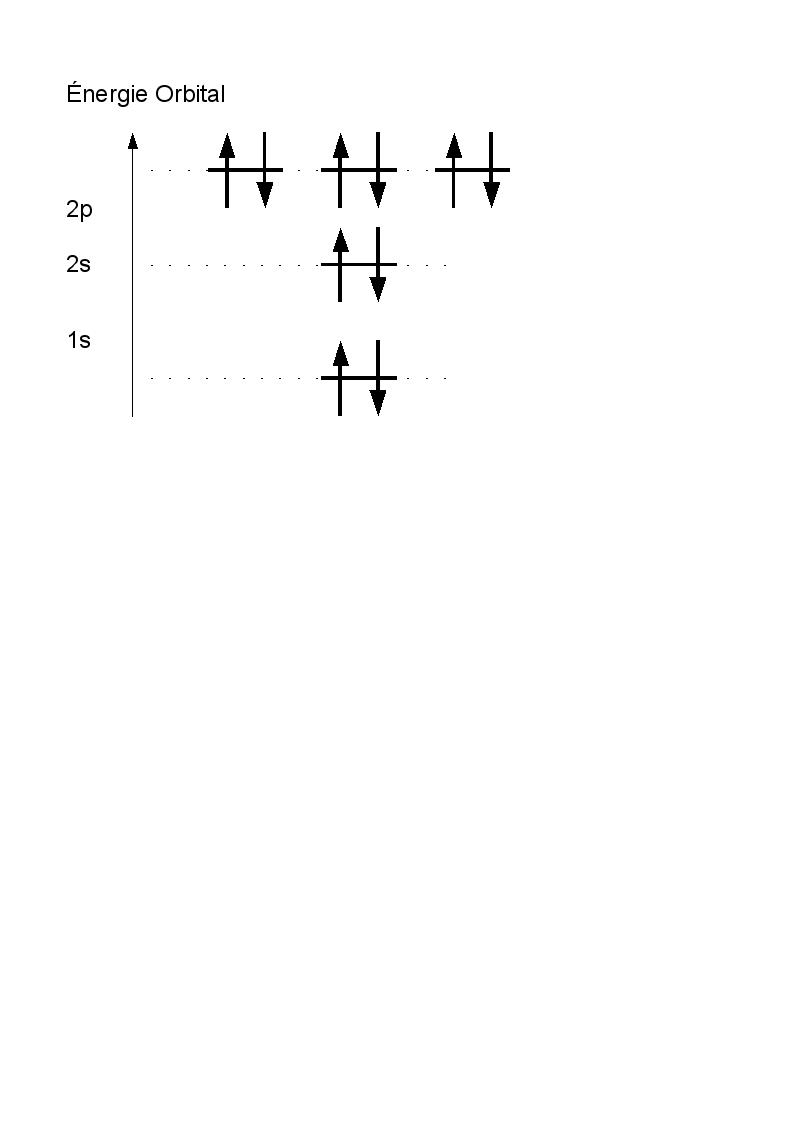
\includegraphics[width=4cm]{configuration.jpg}
%  \caption{Diagramme énergétique}
%\end{figure}
On écrit cette configuration électronique sous la forme :
$$O(Z = 8) : 1s^2 2s^2 2p^4$$
On défini deux états :
\begin{itemize}
 \item[$\rightarrow$] Paramagnètique : Tous les électrons ne sont pas appareillé. Le système peut donc facilement capter ou céder des électrons
 \item[$\rightarrow$] Diamagnétique : Tous les électrons sont appareillé. Le système est "solide"
\end{itemize}
La dernière règle est que quand on rempli une couche dégénérée, on classe toujours, dans la configuration électronique, les élements par valeur de n.
\section{Ionisation d'un atome}
\begin{de}
On appelle énergie de première ionisation $E_{i1}$ l'énergie minimale à fournir pour arracher un électron à un atome gazeux dans son état fondamental \\
Cette énergie est positive, c'est à dire qu'un atome à besoin d'énergie pour perdre un électron, il ne peut pas en céder spotanément.
\end{de}
\chapter{Classification periodique des élements}
\section{Classification periodique de Mendeleiev}
\begin{de}
Les électrons de valence sont les électron dont le nombre quantique principale n est le plus élevé, ainsi que ceux qui appartiennent à des sous-couches en cours de remplissage.
\end{de}
Les éléments sont classé, dans le tableau de Mendeleiev, par ordre croissant de numéro atomique, et d'après leurs propriétés physicochimique. Ces propriétés sont du électrons de valence. Les éléments possèdant les même caractéristique sont classés sur la même colonne
\section{Construction du tableau periodique}
\subsection{Les différents blocs}
\subsubsection{Le bloc s}
Le bloc s est consititué de la première et de le deuxième colonne du tableau periodique. Il rassemble les éléments possèdant une configuration électronique de valence du type : 
$$n.s^x$$
\subsubsection{Le bloc p}
Ce bloc est constitué des 6 dernières colonne, numéroté de 13 à 18. Il rassemble les éléments possèdant une configuration de valence du type : 
$$n.s^2.n.p^x$$
\subsubsection{Le bloc d}
Ce bloc est constitué des 10 colonnes centrale, numéroté de 3 à 12. Il rassemble les éléments possèdant une configuration de valence du type : 
$$(n-1).d^x.ns^2$$
Cependant, ce bloc admet quelques exeptions, qui s'explique du fait de la proximité entre les différents niveaux d'énergie $ns$ et $(n-1).d$.
\subsubsection{Le bloc f}
Ce bloc est le bloc séparé des autres. Il correspond au éléments possédant des électrons de valence dans les orbitale f.
\subsubsection{Propriété}
On remarque, pour les blocs s et p, que le nombre principale n des électrons de valance correspond au numéro de la ligne.\\
La 18 ème ligne rassemble les gaz rares. Ils sont utilisés dans l'expression des configurations électronique, sachant que ceci possède des configurations électronique stable.
\section{Des propriétés}
\subsection{Grandeurs énergétiques}
\subsubsection{Ionisation}
Nous avons défini précédement l'énergie de première ionisation. Elle est positive. On montre, que d'une manière générale, l'énergie d'ionisation augmente de la gauche vers la droite sur une même ligne.
\subsubsection{Affinité électronique}
\begin{de}
On appelle affinité électronique, noté $E_{ae}$, l'énergie libérée par la fixation d'un électron par un atome gazeux. C'est donc la réaction opposé à la réaction de ionisation.\\
Par convention, nous avons : 
\begin{itemize}
 \item[$\rightarrow$] Si la réaction est exothermique, alors $E_{ac}$ est positif
 \item[$\rightarrow$] Si la réaction est endothermique, alors $E_{ac}$ est négatif.
\end{itemize}
On montre aussi que l'affinité électronique augmente de la gauche vers la droite dans le tableau.
\end{de}
\section{Électronégativité}
L'électronégativité, noté $\chi$, est une grandeur relative, adimensionnée, qui détermine l'aptitude d'un atome à attirer les électrons d'une liaison sans influence extérieur. Il existe plusieurs définition pour cette électronégativité. Cependant, quelque soit la définition, l'électronégativité augmente de gauche à droite. 
\subsection{Électronégativité de Pauling}
Cette échelle d'électronégativité repose sur la mesure de l'énergie de dissociation d'une molécule A-B. Considérons la réaction de synthèse de la molécule A-B à partir de $A_2$ et $B_2$. Notons Q le transfert thermique de cette réaction. Pauling nous dit que : 
$$(\chi(A)- \chi(B))^2 = p.|Q|$$
En fixant l'électronégativité de l'hydrogène, on peut déterminer p, et donc déterminer n'importe quelle électronégativité.
\subsection{Électronégativité de Mulliken}
L'électronégativité de l'atome X est définie par la moyenne de l'énergie d'ionisation et de l'affinité électronique de l'atome X, multiplié par un coéfficiant k, qui dépent du système énergétique choisi :
$$\chi(X) = k.\dfrac{E_{i1}(X) + E_{ae}(X)}{2}$$
\subsection{Électronégativité de Allred-Rochow}
Cette définition repose sur la mesure de la force électrostatique exerée par tous les atomes d'une molécule sur le doublet d'une liaison.
\chapter{Structures moléculaires}
\section{Théorie de Lewis}
\subsection{Représentation de Lewis}
La réactivité des atomes est régie par les électrons de valence. La représentation de Lewis permet de mettre ce fait en avant. Elle est défini de la façon suivante : 
\begin{itemize}
 \item[$\rightarrow$] Le noyau et les électrons de coeur (le complément des électrons de valence) sont représenté par le symbole de l'élément.
 \item[$\rightarrow$] Un électron célibataire (dans les électrons de valence) est représenté par un point
 \item[$\rightarrow$] Un doublet d'électron (dans les électrosn de valence) est représenté par un tiret
 \item[$\rightarrow$] La charge d'un composé ionique est entourée par un cercle.
\end{itemize}
À l'aide de cette représentation, on montre par exemple que tous les élements d'une meme colonne ont une représentation de Lewis identique.
\subsection{Liaisons covalentes}
Les atomes se lient entre eux pour se stabiliser. Pour se faire, ils ne sont pas obligé de s'échanger des électrons, ils peuvent se les partager. Dans ce cas, les atomes s'associent pour créer une molécules à liaisons covalentes. Ils y a plusieurs types de liaisons covalentes :
\begin{itemize}
 \item[$\rightarrow$] Liaison covalente simple : Chaque atomes apporte un électron célibataire.
 \item[$\rightarrow$] Liaison covalente de coordination (ou dative) : Les deux électrons de la liaison sont apportés par un seul atomes
\end{itemize}
Les deux électrons constituent un doublet liant. Les atomes peuvent partager un ou plusieurs doublet, pour se stabiliser (tendre vers la configuration d'un gaz rare). Ceci dépend de leurs nombre d'électrons de valence.
\subsection{Valence d'un atome}
\begin{de}
On défini la valence d'un atome (à ne pas confondre avec les électrons de valence) par le nombre de liaisons que peut réaliser un atome dans un édifice polyatomique.
\end{de}
\subsection{Modèle de Lewis}
\subsubsection{Élements chimiques de la première ligne}
La première ligne est composé de deux entités : L'hydrogène et l'hélium. L'hydrogène est monovalent, c'est à dire qu'il ne possède d'un électron de valence, et qu'il ne peut donc réaliser d'une liaison covalente.
\subsubsection{Élements chimiques de la deuxième ligne}
Pour cette deuxième ligne, on défini la règle de l'octet. Dans un édifice polyatomique, les élements chimiques de la deuxième ligne s'entourent au maximum d'un octet, c'est à dire de huit électrons.L'octet est constitué de doublets liants ou non liants.
\subsubsection{Charge formelle}
\begin{de}
Lors de la réalisation d'une liaison covalente de coordination, l'atome possédant le doublet acquiert une charge formelle positive, formelle, car on postule l'egale répartition du doublet. On obtient $Q_f$, la charge formelle, en comparant le nombre d'électron de valence de l'atome isolé, noté $n_v$, et celui de l'atome dans  l'édifice, noté $n_e$ : 
$$Q_f = (n_v - n_e).e$$
Avec e la charge élementaire.
\end{de}
\subsubsection{Éléments chimiques de la troisième ligne}
Pour les élements de cette troisième ligne, on défini la règle de la valence maximale, car les élements de cette ligne ne respecte pas la règle de l'octet.
\begin{de}
La valence maximale d'un atome est égale au nombre d'électrons de valence. Si un atome possède x électrons de valence, il peut s'entourer de 2.x électrons dans un édifice polyatomique.
\end{de}
\subsubsection{Pour les autres lignes}
Dans le cas des autres lignes, on défini la règle des 18 électrons. Dans un édifice polyatomique, les entités chimiques s'entourent au maximum de 18 électrons.
\section{Théorie de la mésomérie}
On montre que la théorie de Lewis à une limitation. En effet, pour le même édifice polyatomique, on peut obtenir plusieurs représentation de Lewis. Il se pose donc la question de savoir laquel est prédominante.
\subsection{Présentation}
Quand un composé est décrit pas plusieurs représentation de Lewis, la théorie de la mésométrie suppose que la configuration éffective de l'édifice résulte d'une moyenne des formules limites. Ceci revient à délocaliser des électrons. C'est à dire que si un édifice polyatomique (par exemple deux atomes) possède par exemple deux représentations de Lewis, qui sont distinct d'un électron, on suppose que l'électron différent est délocalisé, c'est à dire qu'il est réparti sur les deux atomes en même temps.